%%%%%%%%%%%%%%%%%%%%%%%%%%%%%%%%%%%%%%%%%
% Junior dev CV
% LaTeX Template
% CM (Cinna.Monovic@gmail.com)
% 16.10.20
%
% based on the 'developer CV' template by Jan Vorisek (jan@vorisek.me)
%
%%%%%%%%%%%%%%%%%%%%%%%%%%%%%%%%%%%%%%%%%

%----------------------------------------------------------------------------------------
%	PACKAGES AND OTHER DOCUMENT CONFIGURATIONS
%----------------------------------------------------------------------------------------

\documentclass[9pt]{developercv} % Default font size, values from 8-12pt are recommended
\usepackage{hyperref}
\usepackage{xcolor}
\usepackage[most]{tcolorbox}
\usepackage{lipsum}

\begin{document}


%%%   DEFINITION OF COLOR PALLETE (credit goes to www.canva.com for inspiration.)  %%%
%%%   these definitions allow for quick changes of the color pallette, all the colors in      %%%
%%%   the document are defined by these (except for black and white for texts)             %%%
%%%   background colors of colorboxes are defined as a first argument of \tcolorbox      %%%

\definecolor{primary_dark}{HTML}{aec086}
\definecolor{primary}{HTML}{d2d6a8}
\definecolor{complement}{HTML}{8f0a0b}
\definecolor{secondary_dark}{HTML}{291a2d}
\definecolor{secondary}{HTML}{8aa15f}


%%%  Main tcolorbox settings %%%

\tcbset{colback=primary_dark,  % main box background color
			colframe=secondary_dark, % main box frame color
			width=\linewidth, % main box width 
			left=0pt, 
			right=0pt, 
			boxrule=1pt, % frame width
			before=,after=\hfill}

\begin{tcolorbox}


%----------------------------------------------------------------------------------------
%	TITLE AND CONTACT INFORMATION
%----------------------------------------------------------------------------------------

\colorbox{secondary} {\begin{minipage}[t]{0.45\textwidth} 
	\vspace{-\baselineskip} % Required for vertically aligning minipages
	\vspace{10pt}	
	\colorbox{secondary_dark}{{\HUGE\textcolor{complement}{\textbf{\MakeUppercase{Steve}}}}} % First name
	
	\colorbox{secondary_dark}{{\HUGE\textcolor{white}{\textbf{\MakeUppercase{Gates}}}}} % Last name
	\vspace{6	pt}
	
	\colorbox{secondary_dark}{\huge\textcolor{white}{Senior Backend Dev}}% current job title
\end{minipage}

 \begin{minipage}[t]{0.275\textwidth} 
	\vspace{-\baselineskip} 
	\vspace{10pt}
	% The first parameter is the FontAwesome icon name, the second is the box size and the third is the text
	% Other icons can be found by referring to fontawesome.pdf (supplied with the template) and using the word after \fa in the command for the icon you want
	\icon{MapMarker}{12}{Earth}\\
	\icon{Phone}{12}{+11 235 813 213}\\
	\icon{At}{12}{\href{mailto:}{SteveGates@applesoft.com}}\\	
	\icon{Globe}{12}{\href{}{applesoft.com}}\\
	\icon{Github}{12}{\href{}{SteveGates}}
\end{minipage}
}
\colorbox{secondary_dark}{\begin{minipage}[t]{\dimexpr0.2\textwidth-2\fboxrule+2\fboxsep\relax} %photo background
	\vspace{-\baselineskip}
	\vspace{11pt}
	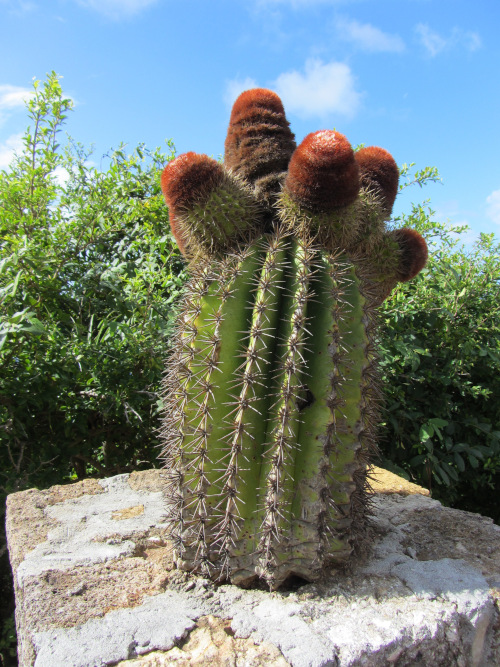
\includegraphics[scale=0.5]{cactus.jpg} % CV photo - if you want the photo and its background to match the width of the first colorbox
																		%you need to scale the image properly using the 'scale' property
	\centering
\end{minipage}
}
\vspace{0.3cm}

%----------------------------------------------------------------------------------------
%	INTRODUCTION, SKILLS AND TECHNOLOGIES
%----------------------------------------------------------------------------------------


\begin{tcolorbox}[colback=primary, 
			colframe=secondary_dark,
			width=\linewidth,
			flush right]
\vspace{-\baselineskip}
\cvsect{Who Am I?}
\vspace{2pt}

\begin{minipage}[t]{0.5\linewidth}
	\vspace{-\baselineskip}
	\vspace{2pt}
	\textcolor{black}{\lipsum[1]}
\end{minipage}
\begin{minipage}[t]{\dimexpr0.4\textwidth+5\fboxrule+10\fboxsep\relax}
	\vspace{-\baselineskip}

	\begin{barchart}{5.5}	%skills barchart (first argument - skill, second - percentage)
		\baritem{C++}{60}
		\baritem{C}{90}
		\baritem{Django}{40}
		\baritem{HTML/CSS}{50}
		\baritem{JavaScript}{20}
		\baritem{SSL}{80}
		\baritem{MySQL}{50}
		\baritem{Rust}{30}
		\baritem{ASP.NET}{70}
	\end{barchart}
\end{minipage}

\end{tcolorbox}

\vspace{0.3cm}

%----------------------------------------------------------------------------------------
%	EXPERIENCE
%----------------------------------------------------------------------------------------


\begin{tcolorbox}[colback=primary, 
			colframe=secondary_dark,
			width=\linewidth]
\vspace{-\baselineskip} 
\cvsect{Work Experience}
\begin{entrylist}
	
	\entry
		{2018 -- 2019\\\footnotesize{some project}} %time and type of work
		{Position1} %position
		{project-website1@project.com} %website/reference
		{This is a project description. I did many important things that led to other important things in this project.\\ \texttt{technology1}\slashsep\texttt{technology2}\slashsep\texttt{technology3}\slashsep\texttt{technology4}\slashsep\texttt{technology5}\slashsep\texttt{technology6}} %details along with technologies used
		\entry
		{2016 -- 2018\\\footnotesize{some project}} %time and type of work
		{Position2} %position
		{project-website1@project.com} %website/reference
		{This is a project description. I did many important things that led to other important things in this project.\\ \texttt{technology1}\slashsep\texttt{technology2}\slashsep\texttt{technology3}\slashsep\texttt{technology4}\slashsep\texttt{technology5}\slashsep\texttt{technology6}} %details along with technologies used
		\entry
		{2012 -- 2016\\\footnotesize{some project}} %time and type of work
		{Position3} %position
		{project-website1@project.com} %website/reference
		{This is a project description. I did many not-so important things in this project cause I was young back then.\\ \texttt{technology1}\slashsep\texttt{technology2}\slashsep\texttt{technology3}\slashsep\texttt{technology4}\slashsep\texttt{technology5}\slashsep\texttt{technology6}} %details along with technologies used
\end{entrylist}

\end{tcolorbox}
\vspace{0.3cm}
%----------------------------------------------------------------------------------------
%	EDUCATION
%----------------------------------------------------------------------------------------

\begin{tcolorbox}[colback=primary, 
			colframe=secondary_dark,
			width=\linewidth,
			flush right]
\vspace{-\baselineskip} 
\cvsect{Education}

\begin{entrylist}
	\entry
		{2015 -- 2020}
		{PhD}
		{My Fav University}
		{subject: Important computer stuff}
	\entry
		{2013 -- 2015}
		{Master's Degree}
		{My Fav University}
		{thesis: computer stuff}
	\entry
		{2010 -- 2013}
		{Bachelor's Degree}
		{My Fav University}
		{thesis: computer stuff.}
\end{entrylist}
\end{tcolorbox}
\end{tcolorbox}

\newpage

%-------------------------------------------
% EXPERIENCE DETAILS
%-------------------------------------------

%This section serves as an expansion of the data filled above. If you want your potential employer to know 
%exactly what do you mean by "I know Linux on 60%" then this is a place where you can specify


\begin{tcolorbox}[]
%----------------------------------------------------------------------------------------
\begin{tcolorbox}[colback=secondary, colframe=secondary_dark, top=-10pt, bottom=0pt, valign=center, halign=center]
\cvsect{Experience Details} 
\end{tcolorbox}
\vspace{8pt}
\begin{detentrylist}
	\detentry
		{Technology} %name
		{\texttt{I can do this }\slashsep\texttt{and this}\slashsep\texttt{and also this}} %specific skills
		{Here I provide details about my experience with the technology (projects, courses, knowledge - anything that feels valuable).} %description
	
	\detentry
		{Technology} %name
		{\texttt{I can do this }\slashsep\texttt{and this}\slashsep\texttt{and also this}} %specific skills
		{Here I provide details about my experience with the technology (projects, courses, knowledge - anything that feels valuable).} %description
		
		\detentry
		{Technology} %name
		{\texttt{I can do this }\slashsep\texttt{and this}\slashsep\texttt{and also this}} %specific skills
		{Here I provide details about my experience with the technology (projects, courses, knowledge - anything that feels valuable).} %description
		
		\detentry
		{Technology} %name
		{\texttt{I can do this }\slashsep\texttt{and this}\slashsep\texttt{and also this}} %specific skills
		{Here I provide details about my experience with the technology (projects, courses, knowledge - anything that feels valuable).} %description
		
		\detentry
		{Technology} %name
		{\texttt{I can do this }\slashsep\texttt{and this}\slashsep\texttt{and also this}} %specific skills
		{Here I provide details about my experience with the technology (projects, courses, knowledge - anything that feels valuable).} %description
		 
		 \detentry
		{Technology} %name
		{\texttt{I can do this }\slashsep\texttt{and this}\slashsep\texttt{and also this}} %specific skills
		{Here I provide details about my experience with the technology (projects, courses, knowledge - anything that feels valuable).} %description
		
		\detentry
		{Technology} %name
		{\texttt{I can do this }\slashsep\texttt{and this}\slashsep\texttt{and also this}} %specific skills
		{Here I provide details about my experience with the technology (projects, courses, knowledge - anything that feels valuable).} %description
		
		\detentry
		{Technology} %name
		{\texttt{I can do this }\slashsep\texttt{and this}\slashsep\texttt{and also this}} %specific skills
		{Here I provide details about my experience with the technology (projects, courses, knowledge - anything that feels valuable).} %description
				
\end{detentrylist}

%%%%%%%%%%%%%%%%%%%%%%%%%%%%%%%%%
% when you run out of space on your page, you need to manually start a new one. tcolorbox won't automatically
% switch to the new page. 
%
%\newpage 				
%\begin{tcolorbox}[]
%\begin{detentrylist}
%	\detentry
%		{Technology} %name
%		{\texttt{I can do this }\slashsep\texttt{and this}\slashsep\texttt{and also this}} %specific skills
%		{Here I provide details about my experience with the technology (projects, courses, knowledge - anything that feels valuable).} %description
%
%\end{detentrylist}
%
% If you have a suggestion how to automate this process, the document is available on
% github: (https://github.com/SpookyMermaidOptimizer). You can fork the project and put the necessary code.

\begin{tcolorbox}[colback=primary, 
			colframe=secondary_dark,
			width=\linewidth,
			]

\begin{minipage}[t]{0.3\textwidth}
	\vspace{-\baselineskip} % Required for vertically aligning minipages

	\cvsect{Languages}
	
	\textbf{English} - native\\
	\textbf{Hindi} - proficient\\
	\textbf{Chinese, Russian} - basic\\
\end{minipage}
\hfill
\begin{minipage}[t]{0.3\textwidth}
	\vspace{-\baselineskip} % Required for vertically aligning minipages
	
	\cvsect{Hobbies}

	Computers, computers, computers, some other things, computers, computers
\end{minipage}
\hfill
\begin{minipage}[t]{0.3\textwidth}
	\vspace{-\baselineskip} % Required for vertically aligning minipages
	
	\cvsect{Other Activities}
	
	Drawing, writing, music, art, theater, opera, other stuff
\end{minipage}

\end{tcolorbox}


\end{tcolorbox}




%%%%%%%%% OTHER MINIPAGES %%%%%%%%%%%%

\end{document}
